\chapter{Evaluation}

This chapter is divided into the evaluation of the quantitative metrics captured by the implementation of this thesis and the network analysis of the graph, which can be generated out of the graph database and further analysed.

All previously described implementations were wrapped into individual docker containers, to first and foremost adopt "Infrastructure as Code", but also to use Kubernetes as scaleable infrastructure. The setup was running on a self hosted Kubernetes cluster using 5 baremetal machines, consisting of 2 master nodes and a total of 5 worker nodes, including the master nodes.

The graph database was occupying one of the 5 worker nodes, using a special taint to only schedule the database on this single node. Due to the usage of baremetal servers, and extra schedule taints, the local disk was directly mounted into the container to provide faster throughput compared to using a virtual disk. Each individual server provided 8 cores and 16 Gigabyte of memory. Typical cloud offers from Azure, AWS or GCP were not accessible.

The remaining implementations, e.g. Jenkins, the crawler and the proxy were all scheduled across the remaining 4 nodes.

The byte range of 0 bytes to 384.000 bytes were crawled within two weeks and no additional crawling was done afterwards, meaning the results are purely from one run, which covered all possible bytes that GitHub allows. The analysis took another two weeks and was done after the two weeks of crawling the results to not overload the graph database. The reasoning for this will be explained further down below.

Considering the crawler implementation one can compare the total amount of available "docker-compose" files that the GitHub API provides to the total amount the crawlers have crawled. As already described in the contribution about the crawler \todo{add reference to chapter}, the GitHub API has some limitations that affect the implementation as well. While providing a horizontally scaleable solution, which is only limited by the amount of GitHub tokens supplied, the GitHub API still has some nowhere described complications. This thesis and included test execution were all done under the terms of the GitHub Terms of Services, which states that the crawling of public data is only allowed for scientific works and require the results to be public \todo{quote TOS}. The TOS also states that the usage of the GitHub API is only allowed with a fair usage in mind, meaning one is not allowed to differ too much of the average usage of certain GitHub API routes. Not complying with those rule will likely result in a termination of ones account. During the data collection period, a total of three GitHub accounts were created with the sole purpose of crawling public data, which is only available with a valid GitHub account. Due to the excessive usage of the code search GitHub API route one out of three accounts received a so-called shadow ban. A shadow ban is a system to hide the fact that the user received a temporary termination. A shadow banned user can still use every GitHub API, but the results returned by the API are always empty even though they still conform the expected schema. GitHub as a provider of this free service does not provide any additional documentation about this system. It is not known at which point the account received the shadow ban, but it is to assume that this limitation was applied after the crawling period of two weeks, since the crawler still reported valid results back compared to two weeks later.

Besides this limitation the only other limiting factor was the 16 Gigabyte of memory for a graph database, which turned out to be not an issue by the memory itself, but the graph database had some blocking operations in the write process, which was heavily relied on. In a recent version this issue was fixed. This issue might have had an impact on the total amount of crawled files, since the database started to block any further insertions. To detect those issues a service called Sentry\footnote{https://sentry.io} was used, which sent alerts for not handled issues like the blocking of the database. This might have had an implication on the total amount of crawled files. The community edition of Grakn does not provide any Kubernetes manifests, thereby, manifests and settings have to be created by oneself, which likely results in a not entirely production ready setup, since the production ready setup with multi sharding is only reserved for the commercial usage.

In the following the actual amount of crawled entries will be compared to the possible and total amount of crawled items that the GitHub API returns. Both will be compared to each other by using a column chart.

\begin{figure}[H]
    \centering
    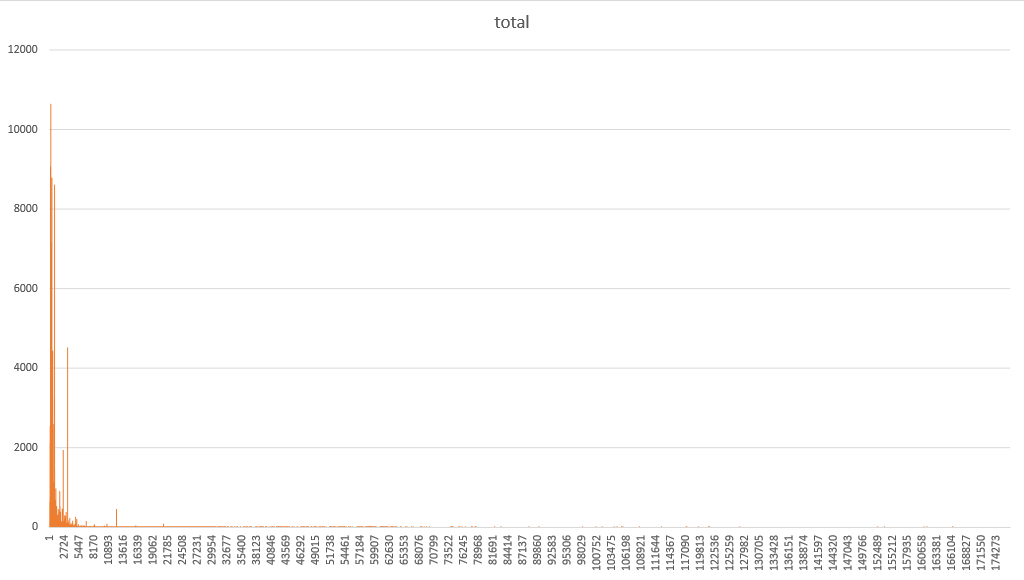
\includegraphics[scale=0.5]{graphics/stats_total.png}
    \caption{Chart representing the total amount of possible results using the GitHub API for the term "docker-compose"}
    \label{fig:stats_total}
\end{figure}

The chart \ref{fig:stats_total} represents the total amount of possible results for the term "docker-compose" using only the GitHub API. The Y-Axis represents the total amount of found occurrences and the X-Axis represents bytes. For this graphical representation the range from 0 to 175.000 was used, since between 175 Kilobyte and 384 Kilobyte are only an additional 200 results. There is a total of 1,1 million results in the chart, most of them clustered around the file size of 100 to 200 bytes, which can be explained due to "docker-compose" files being rather simple and short compared to other deployment scripts. 

\begin{figure}[H]
    \centering
    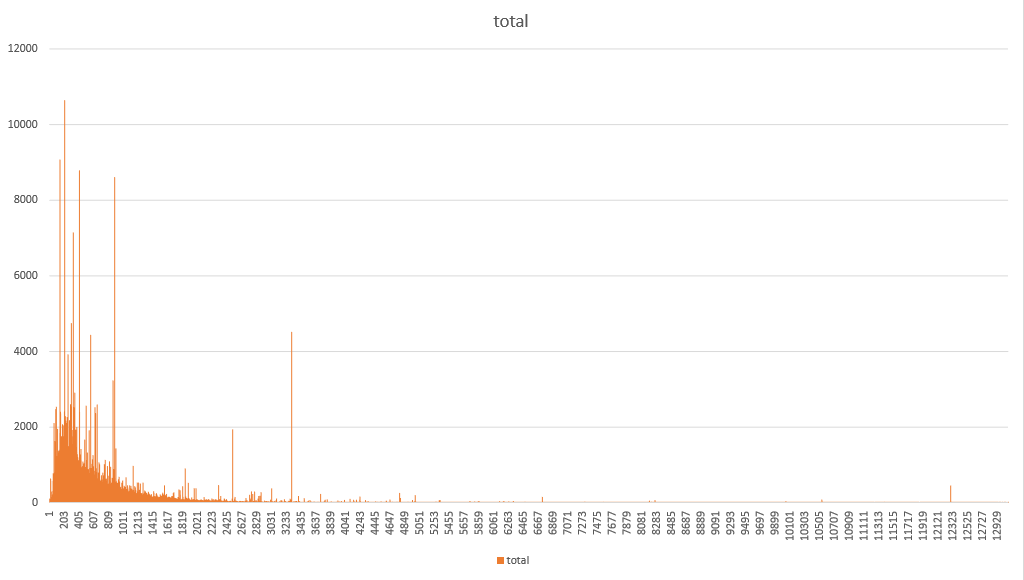
\includegraphics[scale=0.5]{graphics/stats_range.png}
    \caption{Cutout from \ref{fig:stats_total} for the range from 0 to 3000 bytes }
    \label{fig:stats_range}
\end{figure}

The cutout from the range 0 to 3000 bytes as seen in figure \ref{fig:stats_range} shows that the most files are in a range from 100 to 400 bytes and then slowly traverses towards 0, with as seen in figure \ref{fig:stats_total} occasional occurrences in a higher byte range. Both charts \ref{fig:stats_total} and \ref{fig:stats_range} represent the best case if GitHub would return more than a 1000 results for a single query and are both incomplete as well, since GitHub will only return the amount of found results till it receives a timeout. Meaning that running the same query twice would likely result in different results, as the API receives a timeout and returns all found results so far. This behaviour occurs as well when querying single pages, since GitHub only allows a maximal result of 100 entries. This could mean that for running one query on page 10 one could receive a 100 results and for another one close to 0, since the API received a timeout before. In case of this thesis this issue was dismissed, as the author has no influence on the actual implementation of GitHub and it could be mitigated by running the crawling process multiple times for the same bytes.

\begin{figure}[H]
    \centering
    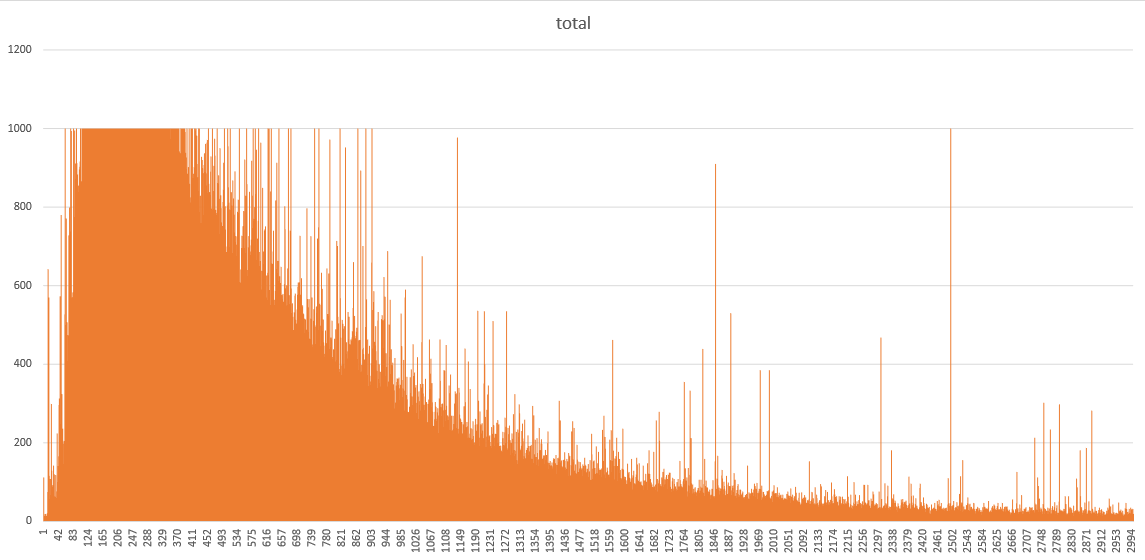
\includegraphics[scale=0.5]{graphics/stats_range_max_possible.png}
    \caption{Cutout from \ref{fig:stats_total} for the range from 0 to 3000 bytes, but a maximum of 1000 results }
    \label{fig:stats_max_possible}
\end{figure}

The chart in figure \ref{fig:stats_max_possible} shall represent the maximum amount of possible results, that can be crawled, since the GitHub API only returns a maximum of 1000 results for a single query. As explained prior for the chart \ref{fig:stats_range}, this does not mean that one will receive a 1000 results, since the GitHub API is nondeterministic.

Further on, the charts for the actual crawled data will be shown, which resulted in 140.000 valid deployments. Valid, since only parseable deployment files were inserted into the database, see \todo{add reference to the explanation in contribution} in the chapter about the implementation.

\begin{figure}[H]
    \centering
    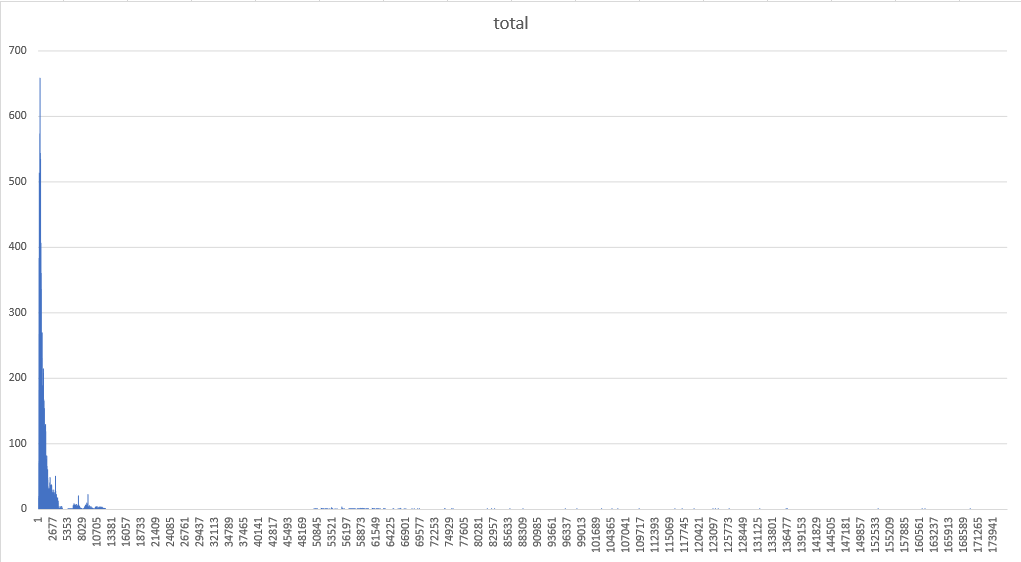
\includegraphics[scale=0.5]{graphics/deployment_stats_total.png}
    \caption{Chart representing the total amount of possible results using the crawler implementation for the term "docker-compose"}
    \label{fig:deployment_total}
\end{figure}

Comparing the figure \ref{fig:stats_total} and the figure \ref{fig:deployment_total}, one may notice a similar representation, which validates the overall implementation, since clusters for similar bytes were successfully crawled with occasional results in the higher byte area.
The chart \ref{fig:deployment_total} also shows that the maximum crawleable number of a 1000 results was never reached, which could be explained by either the nondeterministic behavior of the GitHub API or the blocking process of the database. On the other hand this could simply be explained by non parseable deployment scripts as well, since a lot of people have especially in the lower byte range scripts that are the bare minimum or contain syntactical issues, which cause the parsing to fail and at the same time render the file useless for the "docker-compose" executable as well, since it can not parse the file either.

\begin{figure}[H]
    \centering
    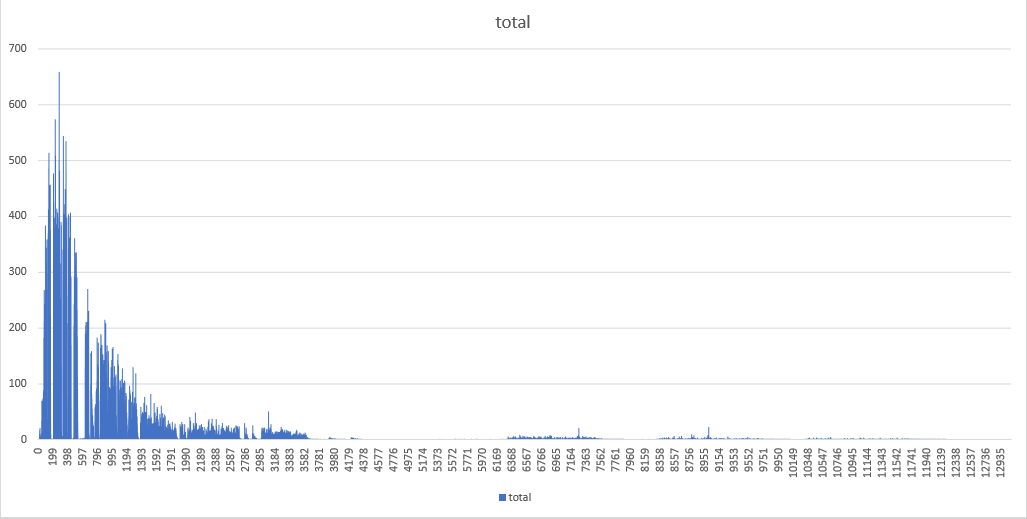
\includegraphics[scale=0.5]{graphics/deployment_stats_range.png}
    \caption{Cutout from \ref{fig:deployment_total} for the range from 0 to 3000 bytes}
    \label{fig:deployment_range}
\end{figure}

The chart \ref{fig:deployment_range} still resembles the chart \ref{fig:stats_range}, but it is visible that that the previously described shadow ban has occurred earlier than expected, since the chart \ref{fig:deployment_range} shows multiple spots where barely any results were returned, e.g. 161-201, 441-481 or 521-641, which mirror the system of a shadow ban. The implementation featured crawler windows, which consisted of a byte range that were individually assigned to each crawler, which in this case could have been assigned to the shadow banned account. During the execution period it was not visible that the account was affected, since it acted as expected and returned results according to the schema.

Overall the GitHub API returned a total amount of 940.000 possible crawleable entries, which can still differ in numbers when actually crawled for due to the way the GitHub API works. A total of 140.000 valid deployment scripts were inserted into the database, which represents 15\% of the total crawleable amount. Limiting factors were in this case the nondeterministic behavior of the GitHub API, the shadow ban system of GitHub and the blocking operations of the graph database. Except the nondeterministic behavior of the GitHub API all other issues can be mitigated for future work, by providing more valid GitHub tokens, which can be switched in case of shadow banned accounts and a more non-blocking graph database. Grakn already provided a patch to resolve the blocking issue, but in the non community edition the graph database can be scaled across multiple Kubernetes nodes as well, since the community edition does not provide any Kubernetes manifests and relied on the implementation of the author.

In total the graph database contains 4,2 million entries, which can be divided into roughly a million nodes, a million edges and two million attributes. Which can be further split down as follows:

\begin{table}[h!]
    \centering
    \begin{tabular}{ |c|c| }
    \hline
    Type & Amount \\
    \hline
         count & 4.279.664 \\
         attributes & 2.546.547 \\
         \hline
         nodes & 836.337 \\
         \hline
         user & 127.084 \\
         repository & 160.506\\
         deployment & 139.469\\
         service & 409.277\\
         \hline
         edges & 896.780 \\
         \hline
         own & 159.834 \\
         contain & 194.797 \\
         include & 404.736 \\
         depend & 137.412 \\
    \hline
    \end{tabular}
    \caption{Graph Database total counts}
    \label{graph_database_total_counts}
\end{table}

The approximately 400.000 services can be analysed further by having a look at the most used images and their versions. This will be divided into multiple tables with different categories, which are databases, programming languages and miscellaneous.

\begin{table}[h!]
    \centering
    \begin{tabular}{ |c|c| }
    \hline
    Image & Amount \\
    \hline
         postgres & 20074 \\
         mysql & 16103 \\
         redis & 13817 \\
         mongo & 11843 \\
         mariadb & 3241 \\
    \hline
    \end{tabular}
    \caption{Top 5 image counts for databases}
    \label{table_image_databases}
\end{table}

\begin{table}[h!]
    \centering
    \begin{tabular}{ |c|c| }
    \hline
    Image & Amount \\
    \hline
         node & 2346 \\
         php & 1121 \\
         golang & 375 \\
         python & 353 \\
         java / openjdk & 325 \\
    \hline
    \end{tabular}
    \caption{Top 5 image counts for programming languages}
    \label{table_image_languages}
\end{table}

\begin{table}[h!]
    \centering
    \begin{tabular}{ |c|c| }
    \hline
    Image & Amount \\
    \hline
         nginx & 8459 \\
         rabbitmq & 3241 \\
         hyperledger/fabric-peer & 2834 \\
         phpmyadmin/phpmyadmin & 2523 \\
         hyperledger/fabric-ca & 2105 \\
    \hline
    \end{tabular}
    \caption{Top 5 image counts for miscellaneous}
    \label{table_image_misc}
\end{table}



Coming to the distributed analysis where Jenkins was used as a base system for running a predefined test for each "docker-compose" file. The tests were conducted for two weeks with a total amount of 60.000 executed tests. By the end a total of 18.000 scripts were successfully evaluated. The failure reasons of the other 42.000 tests can be viewed from different technical perspectives.

For once, public data was crawled and inserted into the database and GitHub repositories were either deleted or made private within this short time period, which accounts to a total of a 1000 repositories. The whole "docker-compose" file could have been saved in the database, but it only has limited further usage, since docker-compose files usually contain a build directive in the file, meaning without the repository the "docker-compose" file can't be executed and this already accounts for a sixth of the score and the vulnerability scan can not be executed in detail as well, which would be worth a third of the whole score. In the beginning, the proxy was missing a denylist causing the 1000 unavailable repositories to be rerun over and over again, but this was fixed during the analysis period.

Kubernetes was used as container orchestration and, as previously described, was set up on dedicated machines, which means the whole maintenance was included as well. A production ready setup was used for the 5 nodes cluster, but after running a total of approximately 20.000 pods no pods and, therefore, no further tests could be scheduled. It turned out that the etcd storage contained too many objects and started blocking the master nodes, which did not respond to any new requests. This caused the whole cluster to stall, since all requests received a timeout. This happened around the 40.000 mark again, resulting in a lot of aborted tests, as a lot of them had stalled.

Overall most of the Jenkins related issues can be mitigated by using managed Kubernetes clusters by e.g. Azure, AWS or GCP with dedicated node pools, which are only used by the CI system.

The score system, explained in the contribution \todo{add reference}, consists of in total 4 different criteria, with each a different significance for the final score. The first third is split into two sixth, since the criteria evaluated in there are of less importance in comparison to the remaining criteria. One sixth considers where a file can be executed or not. Another sixth covers the file length of the file, since the longer the file the more valuable it seems. One third covers the CVSS score, which considers the vulnerability of an image or in this case the vulnerability score of all included images. The last third covers "docker-compose" related best practices.

\begin{figure}[H]
    \centering
    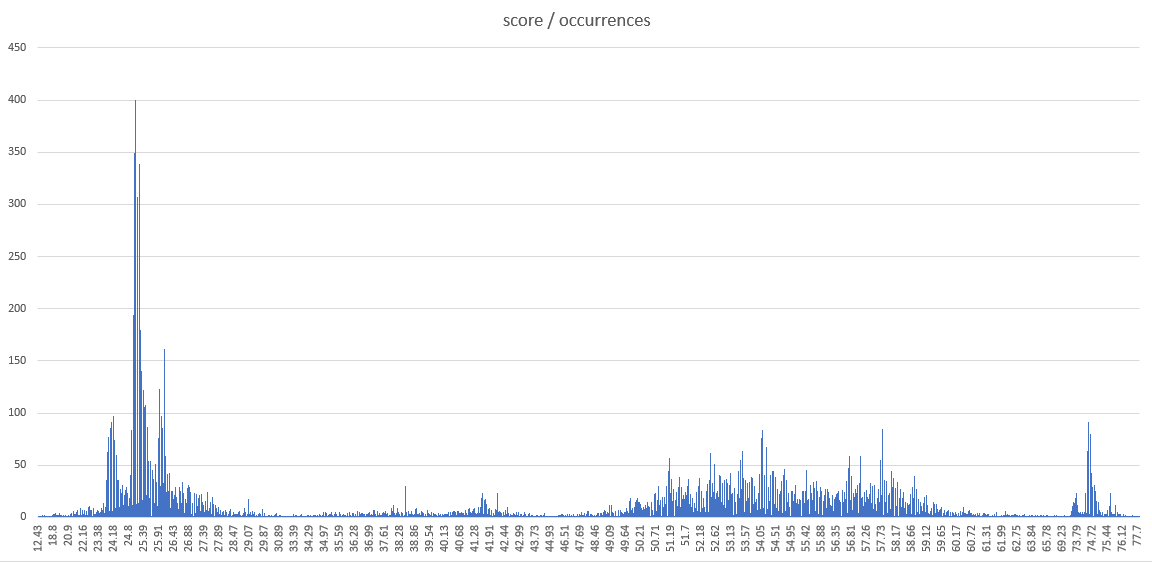
\includegraphics[scale=0.5]{graphics/deployment_score.png}
    \caption{Score distribution}
    \label{fig:deployment_score}
\end{figure}

The figure \ref{fig:deployment_score} shows the score distribution between 0 and 100, where 100 is the best possible score. The X-Axis represents the scores and the Y-Axis are the total amount of occurred scores. The chart shows that there are clusters around the score 24, 54 and 74, which could be explained through the split of the score in four criteria. Some of those criteria are more variable compared to others, e.g. executable is either a true or false and, thereby, contributes either fully or not at all to the score. Taking this fact into account, it's interesting to see that there is no score below twelve, which means that every evaluated deployment script fulfills at least parts of one criteria to the fullest. For the ones around twelve it is to assume that they are executable, since it counts as a sixth of the total score, but at the same time are short and vulnerable. Taking a look at the opposite side of the chart, there is nothing that fulfills a score of a 100, nor is a score close to it. This can be based on the issue of taking the file length too much into account as valuable source, as explained in the contribution part \todo{add reference to part} the file length of 300 as a reference for a "docker-compose" based deployment script might be too much and this unfolds in the chart, since there is a cluster around 74, which will fulfill almost all criteria to the fullest except the file length. For future work this could be changed to the file size, since the file size brings more value compared to the file length. Taking a look at the 180.000 crawled deployment scripts the median of the file length amounts to 22 and even taking the median of the upper part still amounts to 45, meaning that more than 75\% are smaller or equal to the file length of 45. On the other hand taking the file size into account it shows a median of 438 for the 180.000 scripts. This median would have been much more suitable for the score and could be used as a replacement for the file length. Nevertheless, since the file length only accounted for a sixth of the total score and in general has less significance for the value of its content, the score itself and the distribution shown in chart \ref{fig:deployment_score} are still valid and express the importance of the contents of a single deployment script.

\begin{figure}[H]
    \centering
    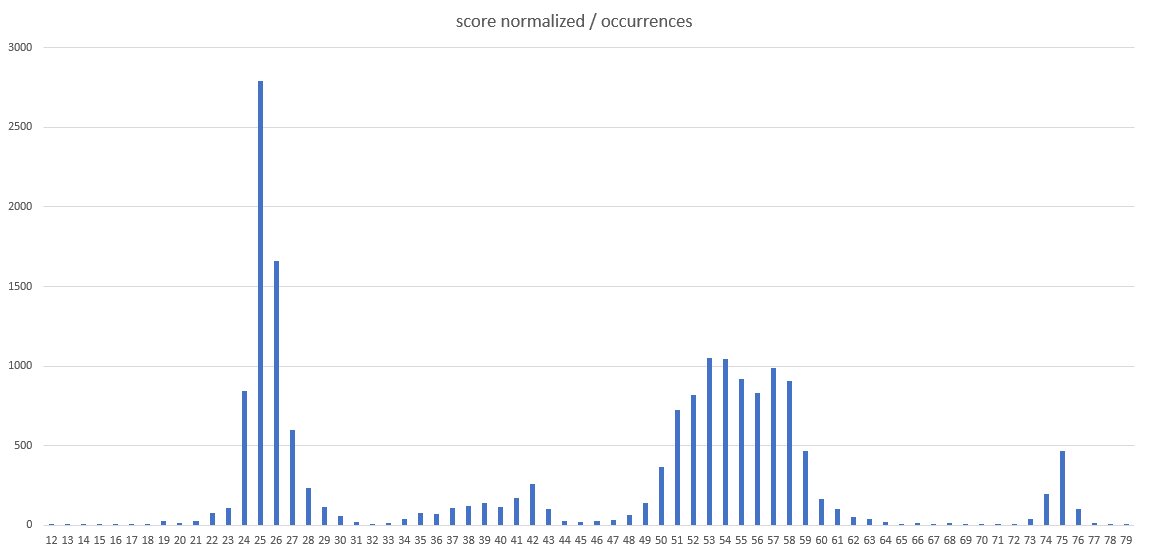
\includegraphics[scale=0.5]{graphics/deployment_score_normalized.png}
    \caption{Score distribution normalized}
    \label{fig:deployment_score_normalized}
\end{figure}

Taking a simplified look at the score distribution in the chart \ref{fig:deployment_score_normalized}, one can see a better picture of the score clusters. For the distribution between the score of 50 and 60 the amount of executable scripts amounts to 99\%, while the total amount of executable files amounts to 56\%. This cluster can be summarized as average but executable, as the deployment script is either fully vulnerable or fully following the best practices or, which is more likely, an average of both criteria.

The CVSS score is the most variable one and looking at the charts of \ref{fig:deployment_score} and \ref{fig:deployment_score_normalized} explain the values inbetween those previously mentioned clusters around the score of 24, 54 and 74.

The score gives an indication whether one script is more valuable compared to another. Still, the suggested scripts should be consumed with caution, since one might not know the contents of one image or the possible dangers of defining specific environment variables without enough care.
For future works the criteria of the file length should be replaced with the file size, as it brings more value compared to the length. The suggestion of using a Z-Score instead of a Min-Max normalization can be dismissed, since the goal of Z-Score normalization is to form the data into a normal distribution, which is not applicable for this type of data. Thereby, the Min-Max normalization is preferred, since the data requires to have the same scale, since one wants to compare across all available data with the same scale.

\begin{table}[h!]
    \centering
    \begin{tabular}{ |c|c|c|c| }
    \hline
    score & image & tag & base image \\
    \hline
         78,69 & linuxserver/letsencrypt & latest & alpine \\
         78,03 & myregistry/simplest-lab & simplestlb, simplestdb, simplestapp & alpine \\
         77,75 & try-webpack & dev & alpine\\
         77,70 & aporeto/apobar & crud & ubuntu \\
         77,53 & python & 3-alpine & alpine\\
         77,53 & traefik & latest & alpine\\
    \hline
    \end{tabular}
    \caption{Images with highest scores}
    \label{images_with_highest_score}
\end{table}

The table \ref{images_with_highest_score} represents the contents of the 5 deployment scripts with the highest score. While the table looks small, some of those images were used multiple times in the same file, making the "docker-compose" files rather complex.
Something that should stick out of the table \ref{images_with_highest_score} is the fact, that most images use alpine as a base image. Alpine compared to other distributions, used for docker, is more secure and simpler, due to the removal of a lot of standard libraries and executables. Due to the removal of such things the resulting image is much smaller and at the same time more secure, since the attack surface is shrinked quite a bit.
The one image that is using Ubuntu in this table is an assumption, since the Dockerfile is not publicly available, nor does the contents of the Docker image give any insights. The image does not contain any executable that one would assume, e.g. ls, echo, cd, shell, bash, and many more. The only thing possible is to gain access to the \$PATH by causing an error, but even this doesn't bring much more information than already known, except for the fact that "snap" is in the path. Snap is a package manager shipped out of the box with newer Ubuntu versions, thereby the assumption of Ubuntu. Nevertheless, this image is much more secure than a default Ubuntu image and shows how to properly secure ones container even against reverse engineering.
Besides alpine as base image, busybox is used quite often as well, since it combines a lot of utilities into a single executable and is perfect for running simple scripts or in the context of Kubernetes as initialization container. Due to its limitied capabilities it's quite secure as well, since there is barely any attack surface.

%Second most important chapter. Verifies the theses defined in the previous chapter. Tries to evaluate and analyze the contribution in qualitative or quantitative terms. Ends with a discussion. Approximately 20 to 30 pages. Can be split into multiple chapters.

% Hier solltest du die limitations deiner Contirbution versuchen zu analysieren. Dies können quantitative sachen sein, wie die limitationen des crawlers wie oft gecrawlet werden kann über github api und wie oft dann andere ergebnisse rauskommen. andere sachen wären zB ob der von dir erstellte score "qualitativ gut" IaC bewerten kann. Für diese unterschiedlichen Punkte sollten folgende Unterpunkte folgen:
%a) Evaluation Setup: hier wird der versuchsaufbau und die durchführung beschrieben. welche größen werden zB gemessen sollte auch beschrieben werden. Womit wird vielleicht das ergebnis verglichen?
%b) Results: Darstellung der Ergebnisse und Beschreibung der Ergebnisse
%c) Discussion: Bewerte die Ergebnisse und ordnete sie ein.
%Am Ende des Kapitels sollte dann eine summary kommen, was der leser gelernt haben soll und welche fragen noch offen geblieben sind für future work und welche forschungsrichtungen man diese arbeit weiter entwickeln kann.

\section{Graph Analysis}
\section{TBD - General Analysis}